\documentclass[12pt]{article}
\usepackage{amsfonts, amssymb, amsmath, amsthm}
\usepackage[margin=1in]{geometry}
\usepackage{tikz}
\usetikzlibrary{patterns, decorations.pathreplacing}

\pagestyle{myheadings}
\markright{Explainer: Rudin 4.6 --- Compact Graphs and Continuity\hfill}

\newcommand{\R}{\mathbb{R}}
\newcommand{\eps}{\varepsilon}

\begin{document}

\begin{center}
    \textbf{\Large Compact Graphs and Continuity}\\[0.5em]
    \large A visual guide to Rudin 4.6
\end{center}

\section{What is the Graph of a Function?}

The \textbf{graph} of $f: E \to \R$ is the set $\{(x, f(x)) : x \in E\} \subset \R^2$.

\begin{center}
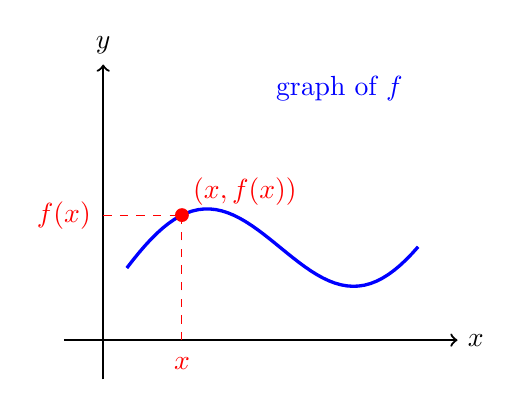
\begin{tikzpicture}[scale=1]
    \draw[thick, ->] (-0.5, 0) -- (4.5, 0) node[right] {$x$};
    \draw[thick, ->] (0, -0.5) -- (0, 3.5) node[above] {$y$};

    % A continuous curve
    \draw[blue, very thick, domain=0.3:4, samples=50] plot (\x, {0.5 + 0.8*sin(80*\x) + 0.3*\x});

    % Some points on the graph
    \fill[red] (1, {0.5 + 0.8*sin(80) + 0.3}) circle (2.5pt);
    \draw[red, dashed] (1, 0) -- (1, {0.5 + 0.8*sin(80) + 0.3});
    \draw[red, dashed] (0, {0.5 + 0.8*sin(80) + 0.3}) -- (1, {0.5 + 0.8*sin(80) + 0.3});

    \node[red] at (1, -0.3) {$x$};
    \node[red] at (-0.5, {0.5 + 0.8*sin(80) + 0.3}) {$f(x)$};
    \node[red] at (1.8, {0.5 + 0.8*sin(80) + 0.3 + 0.3}) {$(x, f(x))$};

    \node[blue] at (3, 3.2) {graph of $f$};
\end{tikzpicture}
\end{center}

\section{The Claim}

\begin{center}
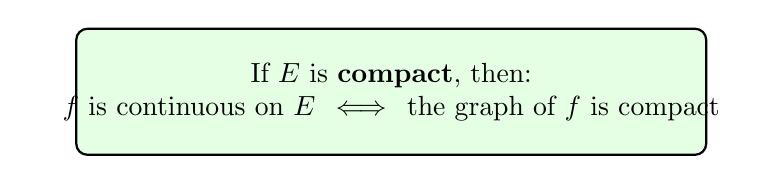
\begin{tikzpicture}[scale=0.8]
    \draw[thick, rounded corners, fill=green!10] (-5, -1) rectangle (5, 1);
    \node[text width=9cm, align=center] at (0, 0) {
        If $E$ is \textbf{compact}, then:\\
        $f$ is continuous on $E$ $\iff$ the graph of $f$ is compact
    };
\end{tikzpicture}
\end{center}

\section{Forward Direction ($\Rightarrow$): Continuous $\implies$ Compact Graph}

\textbf{Key idea:} The map $\varphi: E \to E \times \R$ defined by $\varphi(x) = (x, f(x))$ is continuous.

\begin{center}
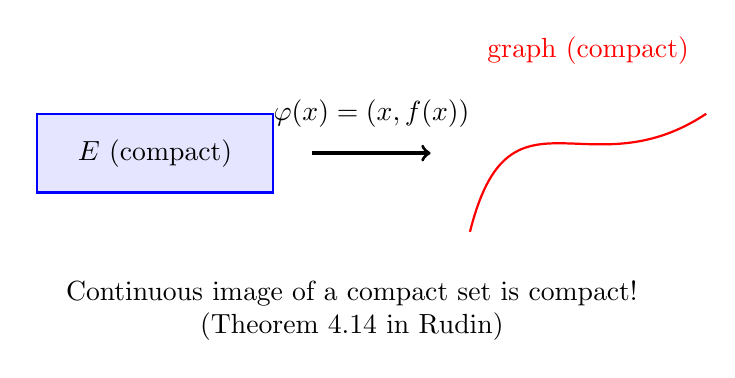
\begin{tikzpicture}[scale=1]
    % E (compact)
    \draw[thick, blue, fill=blue!10] (-4, -0.5) -- (-1, -0.5) -- (-1, 0.5) -- (-4, 0.5) -- cycle;
    \node at (-2.5, 0) {$E$ (compact)};

    % Arrow
    \draw[->, very thick] (-0.5, 0) -- (1, 0);
    \node at (0.25, 0.5) {$\varphi(x) = (x, f(x))$};

    % Graph (compact)
    \draw[thick, red] (1.5, -1) .. controls (2, 1) and (3, -0.5) .. (4.5, 0.5);
    \node[red] at (3, 1.3) {graph (compact)};

    \node[text width=8cm, align=center] at (0, -2) {Continuous image of a compact set is compact!\\(Theorem 4.14 in Rudin)};
\end{tikzpicture}
\end{center}

\textbf{Why is $\varphi$ continuous?}
\begin{itemize}
    \item The first component $x \mapsto x$ is the identity (continuous).
    \item The second component $x \mapsto f(x)$ is continuous by hypothesis.
    \item A map into a product is continuous iff each component is continuous.
\end{itemize}

\section{Backward Direction ($\Leftarrow$): Compact Graph $\implies$ Continuous}

This is the trickier direction. We prove the \textbf{contrapositive}: if $f$ is \emph{not} continuous, the graph is \emph{not} compact.

\begin{center}
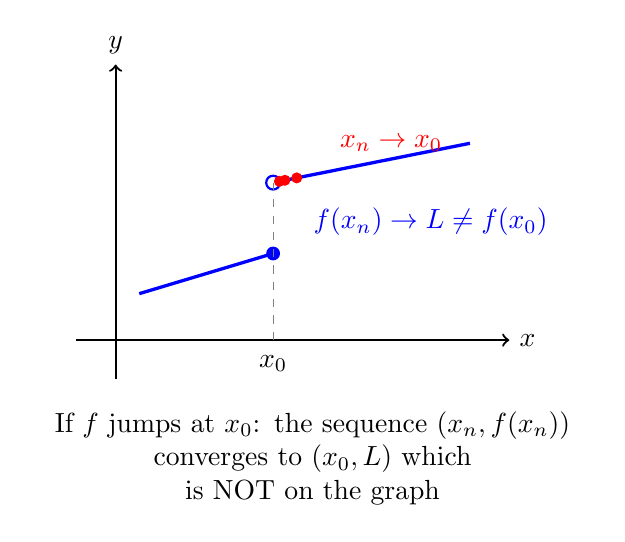
\begin{tikzpicture}[scale=1]
    \draw[thick, ->] (-0.5, 0) -- (5, 0) node[right] {$x$};
    \draw[thick, ->] (0, -0.5) -- (0, 3.5) node[above] {$y$};

    % A discontinuous function
    \draw[blue, very thick, domain=0.3:1.95, samples=30] plot (\x, {0.5 + 0.3*\x});
    \draw[blue, very thick, domain=2.05:4.5, samples=30] plot (\x, {2 + 0.2*(\x - 2)});

    % The jump
    \fill[blue] (2, 1.1) circle (2.5pt);
    \draw[blue, thick, fill=white] (2, 2) circle (2.5pt);

    % x_0
    \node at (2, -0.3) {$x_0$};
    \draw[gray, dashed] (2, 0) -- (2, 2);

    % Sequence
    \fill[red] (2.3, 2.06) circle (2pt);
    \fill[red] (2.15, 2.03) circle (2pt);
    \fill[red] (2.08, 2.016) circle (2pt);

    \node[red] at (3.5, 2.5) {$x_n \to x_0$};
    \node[blue] at (4, 1.5) {$f(x_n) \to L \neq f(x_0)$};

    \node[text width=7cm, align=center] at (2.5, -1.5) {If $f$ jumps at $x_0$: the sequence $(x_n, f(x_n))$\\converges to $(x_0, L)$ which is NOT on the graph};
\end{tikzpicture}
\end{center}

\subsection{The Sequence Argument}

\begin{center}
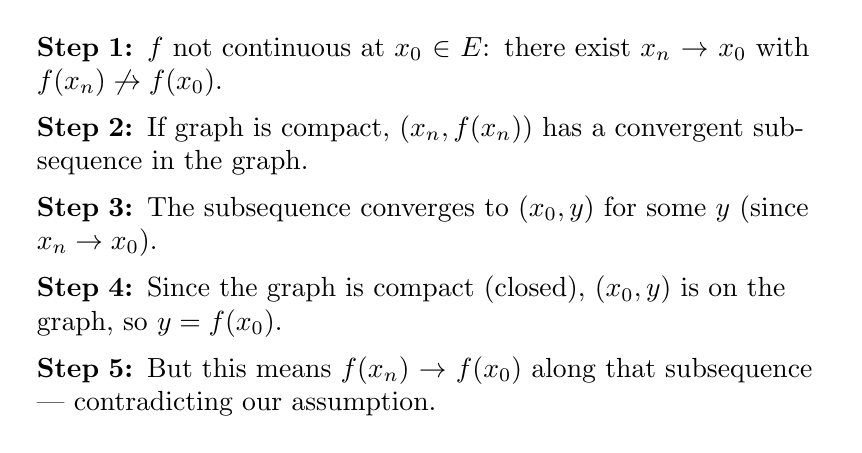
\begin{tikzpicture}[scale=1]
    \node[text width=10cm, align=left] at (0, 0) {
        \textbf{Step 1:} $f$ not continuous at $x_0 \in E$: there exist $x_n \to x_0$ with $f(x_n) \not\to f(x_0)$.\\[0.5em]
        \textbf{Step 2:} If graph is compact, $(x_n, f(x_n))$ has a convergent subsequence in the graph.\\[0.5em]
        \textbf{Step 3:} The subsequence converges to $(x_0, y)$ for some $y$ (since $x_n \to x_0$).\\[0.5em]
        \textbf{Step 4:} Since the graph is compact (closed), $(x_0, y)$ is on the graph, so $y = f(x_0)$.\\[0.5em]
        \textbf{Step 5:} But this means $f(x_n) \to f(x_0)$ along that subsequence --- contradicting our assumption.
    };
\end{tikzpicture}
\end{center}

\section{Why Does Compactness of $E$ Matter?}

Without $E$ compact, the equivalence fails:

\begin{center}
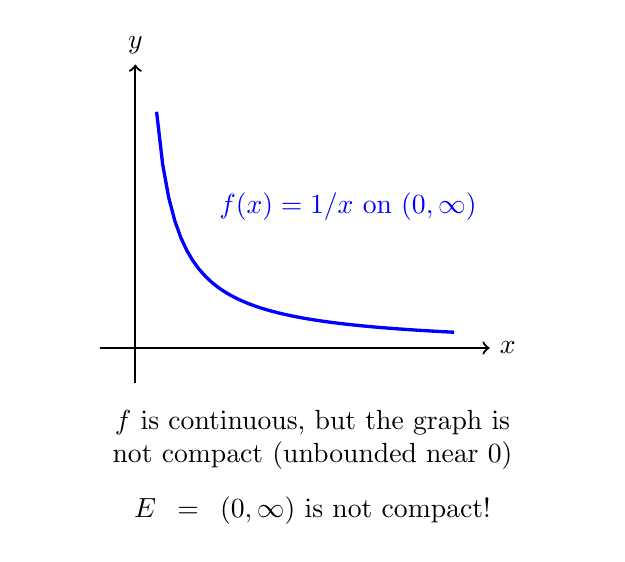
\begin{tikzpicture}[scale=0.9]
    \draw[thick, ->] (-0.5, 0) -- (5, 0) node[right] {$x$};
    \draw[thick, ->] (0, -0.5) -- (0, 4) node[above] {$y$};

    % f(x) = 1/x on (0, infinity)
    \draw[blue, very thick, domain=0.3:4.5, samples=50] plot (\x, {1/\x});

    \node[blue] at (3, 2) {$f(x) = 1/x$ on $(0, \infty)$};

    \node[text width=7cm, align=center] at (2.5, -1.3) {$f$ is continuous, but the graph is\\not compact (unbounded near $0$)};
    \node[text width=7cm, align=center] at (2.5, -2.3) {$E = (0, \infty)$ is not compact!};
\end{tikzpicture}
\end{center}

\section{Summary}

\begin{center}
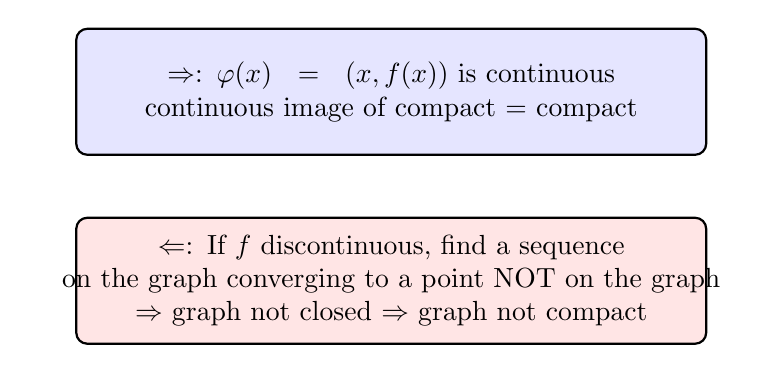
\begin{tikzpicture}[scale=0.8]
    % Forward
    \draw[thick, rounded corners, fill=blue!10] (-5, 1) rectangle (5, 3);
    \node[text width=9cm, align=center] at (0, 2) {
        $\Rightarrow$: $\varphi(x) = (x, f(x))$ is continuous\\
        continuous image of compact = compact
    };

    % Backward
    \draw[thick, rounded corners, fill=red!10] (-5, -2) rectangle (5, 0);
    \node[text width=9cm, align=center] at (0, -1) {
        $\Leftarrow$: If $f$ discontinuous, find a sequence\\
        on the graph converging to a point NOT on the graph\\
        $\Rightarrow$ graph not closed $\Rightarrow$ graph not compact
    };
\end{tikzpicture}
\end{center}

\end{document}
